The model represents the drill string with multiple damped axial and torsional oscillators and the bit with symmetrically arranged blades. The schematic of MDOF model of the drill string is shown in Figure \ref{MDOF_illustration}. The model takes into account damping and
different properties of drill pipe and BHA

\begin{figure}[ht]
  \centering
  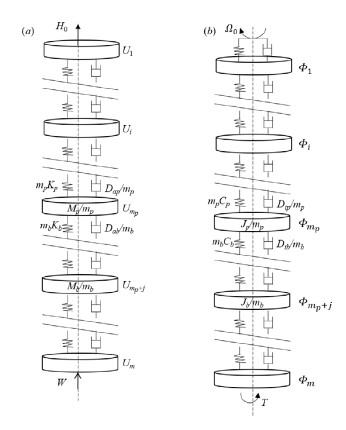
\includegraphics[height=3in]{MDOF_illustration}
  \caption[Schematic of the MDOF model of the drill string]{Schematic of the MDOF model of the drill string. a) axial, b) torsional.}\label{MDOF_illustration}
\end{figure}

The following assumptions are made: 1) The borehole is vertical, 2) Lateral vibration of the drill string are neglected, 3) axial and torsional damping are proportional to the length of drill pipes and BHA, 4) constant hook load and rotary speed from surface (surface boundary conditions). Additionally, the discontinuity of the boundary condition at the bit-rock interface is modeled by
five different regimes classified based on axial, angular velocities, and depth-of-cut, namely, 1) normal drilling, 2) axial stick, 3) loss of contact, 4) torsional stick, 5) backward rotation
The system equations (PDE-ODE coupled) are established from equation of motions (axial and torsional), and bit trajectory function, which is defined to project depth of cut from the angular displacement of the bit. Then,
The PDE-ODE coupled system is numerically solved by discretizing the PDE-ODEs into ODEs. In this study, spectral method with Chebyshev polynomial is applied rather than finite element (FEM) or finite different method (FDM). Spectral method achieved high accuracy for a given number of basis functions and also converged faster compared to other numerical methods. (this is valid with simple geometry). 

Some of the results and potential of the model are summarized below.
\begin{bulletedlist}
  \item Modeling the vibrations of entire drill string (not only the bit).
  \item Possible to conduct frequency analysis since it is multi-degrees of freedom model (\figurename~\ref{StickslipExample}).
  \item It can simulate axial and torsional vibrations including stick-slip event (\figurename~\ref{Axial_torsional_vibration_example}).
  \item Mode analysis can be done by computing the eigenvalues of the linearized system of equation.
  \item Computationally efficient compared to FEM assuming geometrically simple structure.
\end{bulletedlist}

\begin{figure}[ht]
  \centering
  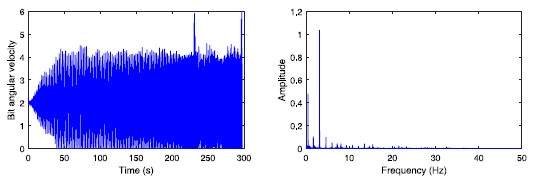
\includegraphics[width=6in]{StickslipExample}
  \caption[Simulation results of bit angular velocity and its frequency spectrum]{Simulation results of bit angular velocity and its frequency spectrum. The result shows the stick-slip occupance due to self-excited torsional vibration}\label{StickslipExample}
\end{figure}


\begin{figure}[ht]
  \centering
  \includegraphics[height=5in]{Axial_torsional_vibration_example}
  \caption[Simulation results showing axial and angular velocity with scaled time]{Simulation results showing axial and angular velocity with scaled time. a) stable regime, b) slow regime of instability, c) fast regime of instability.}\label{Axial_torsional_vibration_example}
\end{figure}

\noindent The following are key questions or points that should be addressed for the model selection.
\begin{bulletedlist}
  \item Can we model deviated or horizontal well?
  \item Geometrical nonlinearity in drill string (for deviated well).
  \item Can we take int to account the effect of contact point?
  \item No lateral vibration - only modeling axial, torsional motion.
  \item Decoupling of axial and torsional vibration. this can be important when it comes to 3D model (i.e., whirling effect).
  \item Current code provided is 2 DOF model.
\end{bulletedlist} 
